\chapter{Theoretical Background}
\section{Basics in Modelling Light in Computer Graphics}
\subsection{Radiometry}
One purpose of Computer Graphics is to simulate the interaction of light with a surface and how a real-world observer, such as a human eye, will perceive this. These visual sensations of an eye are modelled relying on a virtual camera which captures the emitted light from the surface. The physical basis to measure such reflected light is studied under radiometry which deals with measures on the electromagnetic radiation transferred from a source to a receiver. \\

Fundamentally, light is a form of energy propagation, consisting of a large collection of photons, whereat each photon can be considered as a quantum of light that has a position, a direction of propagation and a wavelength $\lambda$. A photon travels at a certain speed $v = c/n$, that depends only the speed of light $c$ and the refractive index $n$ through which it propagates. Its frequency is defined by $f = v/\lambda$ and its carried amount of energy $q$, measured in the SI unit Joule, is given by $q = hf= hv/\lambda n$ where $h$ is the Plank's constant. The total energy of a large collection of photons is hence $Q = \sum_i q_i$.

\subsection{Spectral Energy}

It is important to understand that the human eye is not equally sensitive to all wavelength of the spectrum of light and therefore responds differently to specific wavelengths. Remember that our goal is to model the human visual perception. This is why we consider the energy distribution of a light spectrum rather than considering the total energy of a photon collection since then we could weight the distribution according to the human visual system. So the question we want to answer is: How is the energy distributed across wavelengths of light? \\

One idea is to make an energy histogram from a given photon collection. For this we have to order all photons by their associated wavelength, discretize the wavelength spectrum, count all photons which then will fall in same wavelength-interval, and then, finally, normalize each interval by the total energy $Q$. This will give us a histogram which tells us the spectral energy $Q_{\lambda}$ for a given discrete $\lambda$ interval and thus models the so called spectral energy distribution $\footnote{Intensive quantities can be thought of as density functions that tell the density of an extensive quantity at an infinitesimal by a small interval or a point.}$.

\subsection{Spectral Power}
Rendering an image in Computer Graphics corresponds to capturing the color sensation of an illuminated, target scene at a certain point in time. Each color is associated with either a particular wavelength or is composed of a wavelength spectrum$\footnote{A wavelenght spectrum is a collection of certain wavelengths. For example brown color is a composition of many wavelengths in the region of yellow, orange or read color in combination with low luminance.}$. Thus a color is directly related to a certain amount of energy. In order to determine the color of a to-be-rendered pixel of an image, we have to first get a sense of how much light (in terms of energy) passes through the area which the pixel corresponds to. We begin by considering the flow of energy $\Phi = \frac{\Delta Q}{\Delta t}$ transferred through this area over a unit period of time. This allows us to measure the energy flow through a pixel during a certain amount of time. In general, power is the estimated rate of energy production for light sources and corresponds to the flux. It is measured in the unit Watts, denoted by Q. Since power is a rate over time, it is well defined even when energy production is varying over time. As with Spectral Energy for rendering, we are really interested in the spectral power $\Phi_\lambda = \frac{\Delta \Phi}{\Delta \lambda}$, measured in Watts per nanometer.

\subsection{Spectral Irradiance}
Before we can tell how much light is reflected from a given point on a surface towards the viewing direction of an observer, we first have to know how much light arrives at this point. Since in general a point has no length, area or even volume associated, let us instead consider an infinitesimal area $\Delta A$ around a such a point. Then, we can ask ourself how much light falls in such a small area. Further while observing this process over a short period of time, the measured quantity gives us the the spectral irradiance $E$ as illustrated in figure $\ref{fig:irradiance}$. Summarized, this quantity tells us how much spectral power is incident on a surface per unit area and mathematically is equal:

\begin{equation}
 E_{\lambda} = \frac{\Phi_{\lambda}}{\Delta A}
\end{equation} 

\begin{figure}[H]
  \centering
  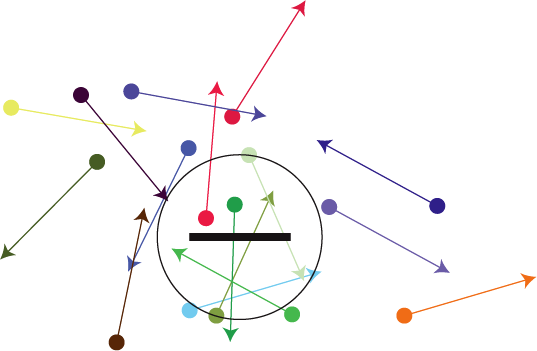
\includegraphics[scale=0.5]{background/irradiance.png}
  \caption[Irradiance]{Irradiance is the summed up radiance over all directions. The black border is representing a surface element.}
  \label{fig:irradiance}
\end{figure}

\subsection{Spectral Radiance}
When rendering an image we have to determine the color of each pixel of the image. Although irradiance tells us how much light is arriving at a point and gets reflected, it tells us nothing about the power distribution across different directions. The direction of the element is important because the human eye may perceive the brightness of an illuminated objects differently when looking from direction. 

\begin{figure}[H]
  \centering
  \subfigure[Radiances is the density of photons per area per solid angle]{
    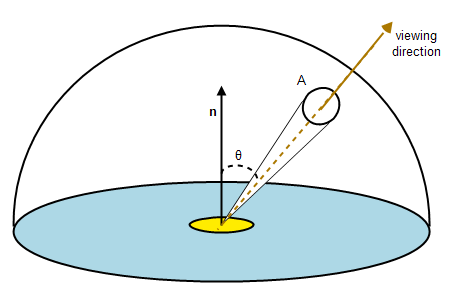
\includegraphics[scale=0.4]{background/radiancehemisphere.png}
    \label{fig:radiance}
  }
~
  \subfigure[Solid angle is the area of a surface patch on a sphere with radius R which is spanned by a set of directions]{  
    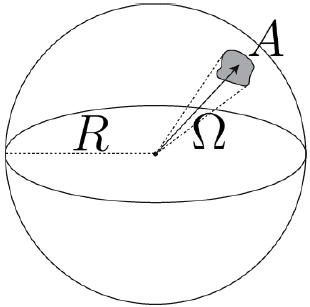
\includegraphics[scale=0.6]{background/solidangle.png}
    \label{fig:solidangle}
  }
\caption[Concept of Radiance]{Illustration of the concepts of radiance and of solid angle and how they are related.}  
\label{fig:radianceBasics}
\end{figure}
\noindent
This concept is described by the radiometric quantity radiance. Basically, radiance is the measure of light energy passing through or emitted from a small area around a point on a surface towards a given direction during a short period in time. More formally this is the spectral power emerging from an arbitrary point (an infinitesimal area around this point) and falls within a given solid angle (see figure$\footnote{Modified from a figure in Computer Graphics class 2012 in chapter \emph{Colors}}$ $\ref{fig:solidangle}$) in a specific direction (usually towards the observer) as shown in figure $\ref{fig:radiance}$. Formally, this leads us to the following mathematical formalism: 

\begin{equation}
 L_{\lambda}(\omega) = \frac{d^2 \Phi_{\lambda}}{dA d\Omega} \approx \frac{\Phi_{\lambda}}{\Omega A}
\end{equation}

where $L$ is the observed spectral radiance in $Wm^-2 sr^-1$ in direction $\omega$$\footnote{The direction $\omega$ is determined by two angles, $\phi$ and $\theta$ like illustrated in figure $\ref{fig:radianceBasics}$}$, $\Theta_{\lambda}$ is the total power emitted, $\theta$ is the angle between the surface normal and the specified direction, $A$ is the area of the surface and $\Omega$ is the solid angle subtended by the observation or measurement. \\

It is useful to distinguish between radiance incident at a point on a surface and excitant from that point. Terms for these concepts sometimes used in the graphics literature are surface radiance $L_r$ for the radiance \textit{reflected} from a surface and field radiance $L_i$ for the radiance \textit{incident} at a surface.  

\subsection{BRDF}
In order to render the colorization of an observed object, a natural question in Computer Graphics is what portion of the incident light a viewer will receive after reflection, after when he looks at an illuminated object. For any given surface which is illuminated from a certain direction $\omega_i$, we can ask ourself how much light is reflected from any point on this surface towards a viewing direction $\omega_r$. This is where the Bidirectional Reflectance Distribution Function (BRDF) comes into play, which is a radiometric quantity telling us how much light is reflected at an opaque surface. Mathematically speaking, the BRDF is the ratio of the reflected radiance pointing in the direction $\omega_r$ to the incident irradiance coming from the inverse direction of $\omega_i$ as illustrated in figure $\ref{fig:brdfillustration}$. Hence the BRDF is a four dimensional function defined by four angles $\theta_i$, $\phi_i$, $\theta_r$ and $\phi_r$.

\begin{figure}[ht]
  \centering
  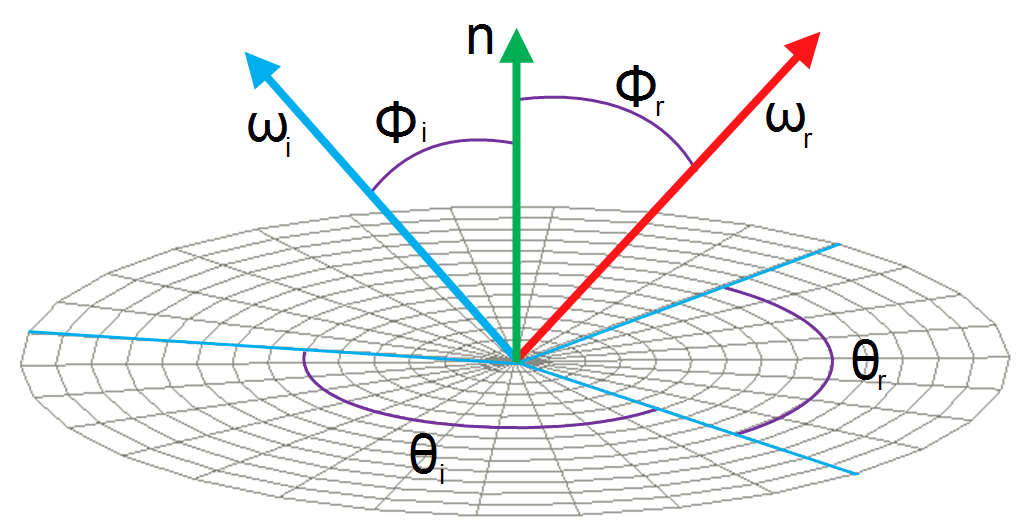
\includegraphics[scale=0.5]{background/mybrdfmodel.png}
  \caption[BRDF Model]{Illustration of the BRDF model, where $\omega_i$ is pointing to the light source and the viewing direction is denoted by $\omega_r$. Both unit direction vectors are defined w.r.t to a surface normal $\mathbf{n}$ for every point on the surface.}
  \label{fig:brdfillustration}  
\end{figure}

Formally, a BRDF for any given wavelength $\lambda$ is defined as:

\begin{align}
  BRDF_{\lambda}(\omega_i, \omega_r)
  & = \frac{dL_r(\omega_r)}{dE_i(\omega_i)} \nonumber \\
  & = \frac{dL_r(\omega_r)}{L_i(\omega_i)cos(\theta_i)d\omega_i}
  \label{eq:defbrdf}
\end{align}

Where $L_{r}$ is the reflected spectral radiance, $E_i$ is the incident spectral irradiance and $\theta_{\text{i}}$ is the angle between $\omega_{\text{i}}$ and the surface normal $\mathbf n$. Also, $L_i$ is the incident spectral radiance.

\subsection{Wavespectrum and Colors}
In order to see how crucial the role of human vision plays, let us consider the following definition of color by \textit{Wyszechkiu and Siles} mentioned in the Fundamentals of Computergraphics Book$\cite{fundcg}$, stating that \textit{"Color is the aspect of visual perception by which an observer may distinguish differences between two structure-free fields of view of the same size and shape such as may be caused by differences in the spectral composition of the radiant energy concerned in the observation"}. Therefore, similarly like the humans' perceived sensation of smell and taste, color vision is just another individual sense of perception giving us the ability to distinguish between different frequency distributions of light which we experienced as different colors.

\begin{figure}[H]
  \centering
  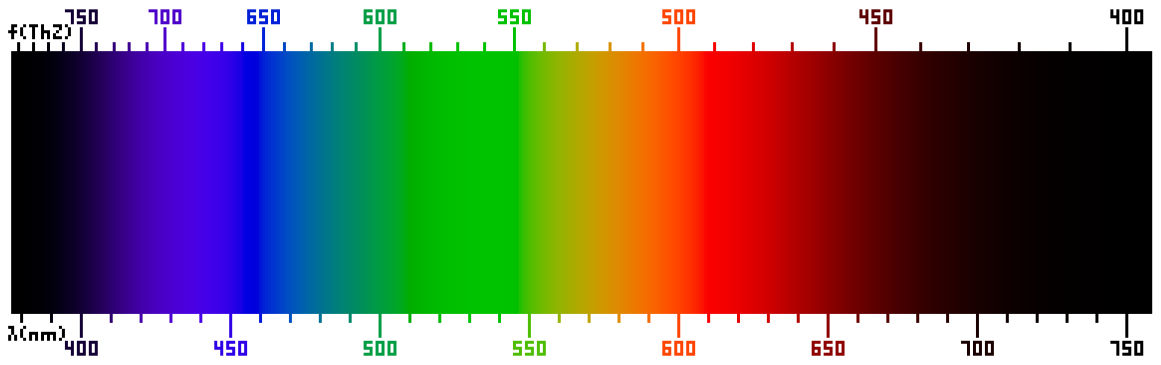
\includegraphics[scale=0.35]{background/lightspec.png}
  \caption[Visible Lightspectrum]{Frequency (top) and wavelength (bottom) of colors of the visible light spectrum$\footnotemark$.}
  \label{fig:colorspectrum}
\end{figure}
\footnotetext{Similar figure like used in computer graphics class 2012 in chapter colors}

In general, an eye consists of photoreceptor cells which are responsible for providing ability of color-perception. A schematic of an eye is illustrated in figure $\ref{fig:humaneye}$. Basically, there are two specialized types of photoreceptor cells, cone cells which are responsible for color vision and rod cells, which allow an eye to perceive different brightness levels.

\begin{figure}[H]
  \centering
  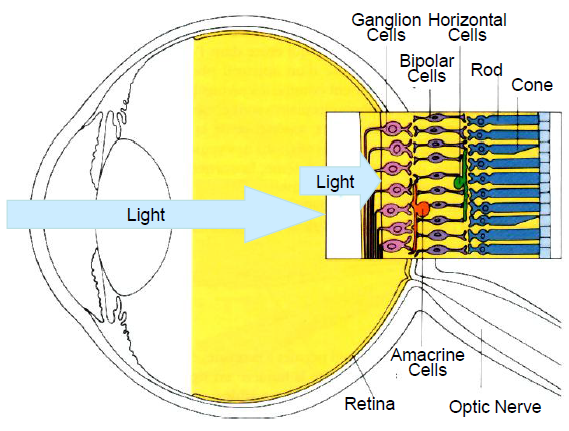
\includegraphics[scale=0.35]{background/humaneye.png}
  \caption[humanayeschematic]{Schematic$\footnotemark$ of photoreceptor cells, cones and rods, in a human eye }
  \label{fig:humaneye}
\end{figure}
\footnotetext{image of illustration has been taken from \\ \texttt{http://en.wikipedia.org/wiki/Bidirectional\textunderscore reflectance\textunderscore distribution\textunderscore function}}

A human eye is made of three different types of cone cells, having their peak sensitivity in different wavelength ranges. More precisely, there are cone cells most sensitive to short wavelengths between $420 nm$ and $440 nm$, those which are most sensitive in the middle range between $530 nm$ and $550 nm$ and those which have their peak in the long range, from $560 nm$ to $580 nm$. Therefore, any color sensation in human color perception can therefore be described by just three parameters, corresponding to the levels of stimulus of these three types of cone cells.  

\subsection{Colorspace}
\label{sec:colorspace}
In order to render accurate images of how a human observer sees its world, a mathematical model of the human color perception is required. Remember that color sensation is due to a visual stimulus processed by cone cells in an eye. A human eye contains three different types of cone cells. Therefore, one possible approach is to describe each kind of these cone cells with a function mapping each wavelength to a certain sensitivity. In the early 1920 from a series of experiments, the so called CIE RGB color space was derived (see figure $\ref{fig:ciergb}$). This space describes the response of cone cells of an average human individual, the so called standard observer. Basically, a statistically sufficiently large number of probands were exposed to different target light colors expressed by their wavelength. The task of each proband was to reproduce these target colors by mixing three given primary colors, red, green and blue light. The strength  of each primary color could be manually adjusted by setting their relative sensitivity. Those adjustment weights have been measured, aggregated and averaged among all probands for each primary color. This model describes each color as a triple of three real valued numbers$\footnote{note that there are  negative color weights possible in the CIE RGB colors space. This is why some human perceived color sensations could not be reconstructed using just an additive color model (adding three positively weighted primary values). Therefore, a probabant was also allowed to move one of the primary colors to the target color and instead was supposed to reproduce this new color mix using the two remaining primaries (subtractive model). The value of the selected, moved primary was then interpreted as being negative weighted in an additive color model.}$, the so called tristimulus values. Summarized, these experiments provided certain weights of primary colors in order to match a color at a certain wavelength according to the average human color perception. However, some of these weights could have a negative value. \\

\begin{figure}[H]
  \centering
  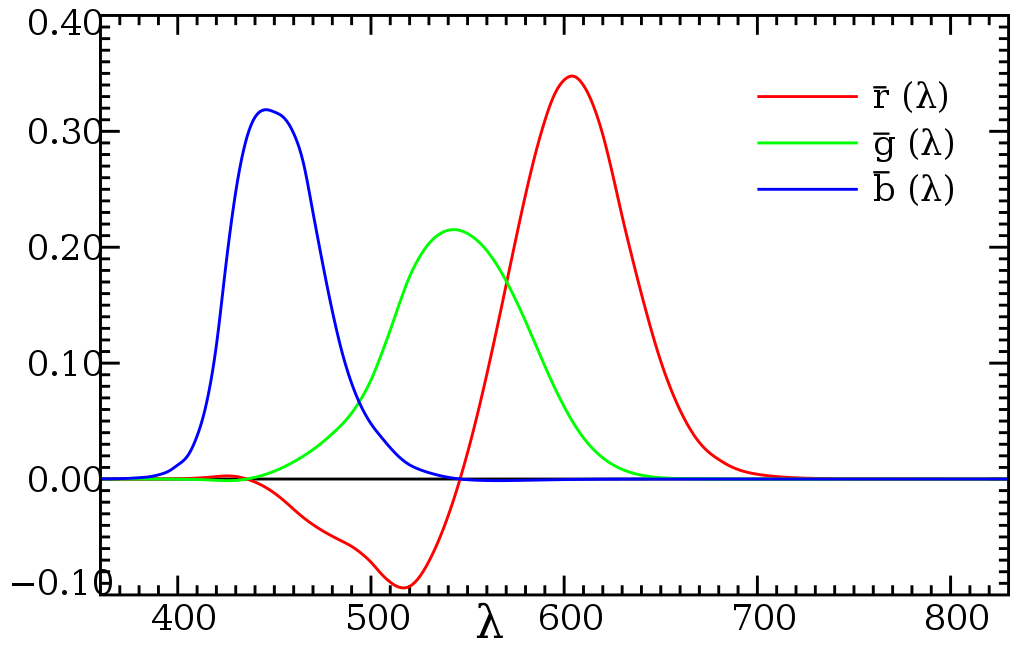
\includegraphics[scale=0.3]{introduction/ciergb.png}
  \caption[CIE RGB Color Matching Functions]{Plots$\footnotemark$ of CIE 1931 RGB Color matching functions showing the amounts of primaries needed to match a certain wavelength.}
\label{fig:ciergb}
\end{figure}
\footnotetext{These plots have been taken from \texttt{http://en.wikipedia.org/wiki/CIE\textunderscore 1931\textunderscore color\textunderscore space}}

The disadvantage of the CIE RGB colorspace is that some of its color weights are negative. Thus, scientist dervied the CIE XYZ colorspace which as no negative color matching functions but is still additive$\footnote{Remember, the property of an additive colorspace is that any color can be represented as a weighted sum of matching functions of that color space.}$. Figure $\ref{fig:matchingfunction}$ visualizes the matching functions of the CIE XYZ space. Another property of the CIE XYZ space is that its Y component is representing the luminance of the corresponding color. Usually, the CIE XYZ space is used as a reference colorspace to define colorspace transformations. \\

Pragmatically speaking, color spaces describe the range of colors a camera can see, a printer can print or a monitor can display. Thus, formally we can define it as a mapping from a range of physically produced colors from mixed light to a standard objective description of color sensations registered in the eye of an observer in terms of tristimulus values. 

\begin{figure}[H]
  \centering
  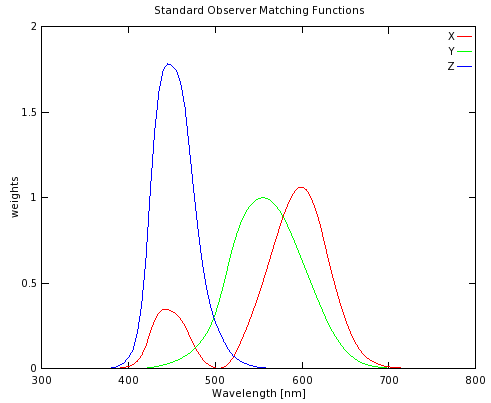
\includegraphics[scale=0.7]{background/somatchingfunctions.png}
  \caption[Color Matching Functions]{Plots of our CIE XYZ color matching functions we used for rendering}
  \label{fig:matchingfunction}
\end{figure}

Interpolating all measured tristimuli values gives us three basis functions, the CIE color matching functions $\overline{x}(\lambda)$, $\overline{y}(\lambda)$, $\overline{z}(\lambda)$. In figure $\ref{fig:matchingfunction}$ are the numerical description of the chromatic response of the observer. They can be thought of as the spectral sensitivity curves of three linear light detectors yielding the CIE tristimulus values X, Y and Z. \\

The tristimulus values for a color with a spectral power distribution $I(\lambda)$, are given in terms of the standard observer by:

\begin{align}
    X= \int_{\Lambda} I(\lambda)\,\overline{x}(\lambda)\,d\lambda \nonumber \\
    Y= \int_{\Lambda} I(\lambda)\,\overline{y}(\lambda)\,d\lambda \nonumber \\
    Z= \int_{\Lambda} I(\lambda)\,\overline{z}(\lambda)\,d\lambda
\label{eq:tristimulusvalues}
\end{align}
\noindent
where $\lambda$ is the wavelength of the equivalent monochromatic light spectrum $\Lambda = [380nm, 780nm]$. Note that it is not possible to build a display that corresponds to the CIE XYZ colorspace. For this reason it is necessary to design other color spaces, which are physically realizable, efficiently encoded, perceptually uniform and have an intuitive color specification. There are simple conversions between XYZ color spaces to other color space - such as the RGB colorspace -  described as linear transformations.

\subsection{Spectral Rendering}
When rendering an image, most of the time we are using colors described in a certain RGB color space. However, a RGB colorspace results from a colorspace transformation of the tristimulus values, which themselves are inherent to the human visual system. Therefore, many physical phenomenon are poorly modelled when they rely on RGB colors for rendering. Using only RGB colors for rendering is like assuming that a given light source emits light of only three particular wavelengths. But in reality this is rarely the case. Spectral rendering refers to using certain wavelength spectrum, for e.g. the human visible light spectrum, instead of simply using only the range of RGB values in order to render an illuminated scene. This captures the physical reality of specific light sources way more accuratly. Keep in mind that even when we make use of a spectral rendering approach, we have to convert the final spectra to RGB color values when we want to display an image on an actual display.

\subsection{Rendering Equation}
As discussed previously, colors are associated to radiance. Since we are starting with Stam's BRDF$\footnote{Remember that a BRDF is the portion of a incident light source reflected off a given surface towards a specified viewing direction.}$ formulation but want to perform a simulation rendering structural colors, we have to reformulate this BRDF equation such that we will end up with an identity of the reflected spectral radiance. This is where the rendering equation comes into play. Let us assume we are given an incoming light source directional at a solid angle $\omega_i$ and $\theta_i$ is its angle of incidence and that $\omega_r$ is the solid angle for the viewing direction. Further let $\lambda$ denote the wavelength$\footnote{Notice that, to keep our terms simple, we have dropped all $\lambda$ subscripts for spectral radiance quantities.}$ and $\Omega$ is the hemisphere of integration for the incoming light. Then, we are able to formulate a $BRDF_\lambda$ by using its definition $\ref{eq:defbrdf}$:  

\begin{alignat}{4}
& f_r(\omega_i, \omega_r) &&= \frac{dL_r(\omega_r)}{L_i(\omega_i)cos(\theta_i)d\omega_i} \nonumber \\
\Rightarrow{} & f_r(\omega_i, \omega_r) L_i(\omega_i)cos(\theta_i)d\omega_i &&= dL_r(\omega_r) \nonumber \\
\Rightarrow{} & \int_{\Omega}f_r(\omega_i, \omega_r) L_i(\omega_i)cos(\theta_i)d\omega_i &&= \int_{\Omega}dL_r(\omega_r) \nonumber\\
L_r(\omega_r) &&= \Rightarrow{} & \int_{\Omega}f_r(\omega_i, \omega_r) L_i(\omega_i)cos(\theta_i)d\omega_i
\label{eq:initialbrdf}
\end{alignat}

The last equation is the so called rendering equation $\label{sec:dirlighsourceassumption}$. We assume that our incident light is a directional, unpolarized light source like sunlight and therefore its radiance is given as 

\begin{equation}
 L_{\lambda}(\omega)=I(\lambda)\delta(\omega-\omega_i)
\label{eq:radiancedirlightsource}
\end{equation}

where $I(\lambda)$ is the intensity of the relative spectral power for the wavelength $\lambda$. By plugging the identity in equation $\ref{eq:radiancedirlightsource}$ into our current rendering equation $\ref{eq:initialbrdf}$, we will get:

\begin{align}
L_{\lambda}(w_r) 
& = \int_{\Omega} BRDF_{\lambda}(\omega_i, \omega_r) L_{\lambda}(\omega_i) cos(\theta_i) d\omega_i \nonumber \\
& = BRDF_{\lambda}(\omega_i, \omega_r) I(\lambda) cos(\theta_i)
\label{eq:deribrdfwithdirsource}
\end{align}

where $L_{\lambda}(\omega_i)$ is the incident radiance and $L_{\lambda}(\omega_r)$ is the radiance reflected by the given surface. Note that the integral in equation $\ref{eq:deribrdfwithdirsource}$ vanishes since $\delta(\omega-\omega_i)$ is only equal one if and only if $\omega = \omega_i$. 

\section{Wave Theory for Light and Diffraction}
\subsection{Basics in Wave Theory}
In order to prepare the reader for relevant concepts in physics which are used later for derivations and reasonings within this thesis, I am going to provide a quick introduction to the basics of wave theory and related concepts. In physics, a wave describes a disturbance that travels from one location to another through a certain medium. The disturbance temporarily displaces the particles in the medium from their rest position which results in an energy transport along the medium during wave propagation. Usually, when talking about waves we are actually referring to a complex valued function which is a solution to the so called \emph{wave equation} which is modelling how the wave disturbance proceeds in space during time. \\

There are two types of waves, (a) mechanical waves which deform their mediums during propagation like sound waves and (b) electromagnetic waves consisting of periodic oscillations of an electromagnetic field, such as light. As illustrated in figure $\ref{fig:wavebasics}$, there are several properties someone can use and apply in order to compare and distinguish different waves:

\begin{figure}[H]
  \centering
  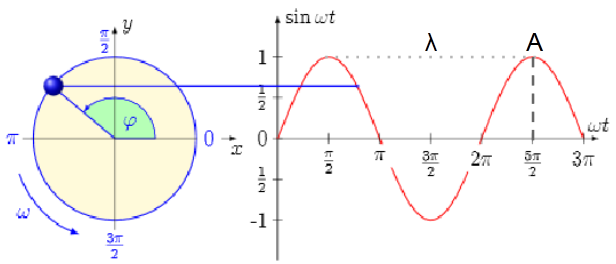
\includegraphics[scale=0.65]{background/waveschematicimpr.png}
  \caption[Sinewave]{Simplified, one dimensionally real valued wave function$\footnotemark$, giving an idea about some important wave properties. We denote the crest of a wave as the highest point relative to the equilibrium line (zero height along time axis) and similarly the trough as the lowest point.}
  \label{fig:wavebasics}
\end{figure}
\footnotetext{Image source: http://neutrino.ethz.ch/Vorlesung/FS2013/index.php/vorlesungsskript}

\begin{description}
  \item[Wavelength:] It ss usually denoted by $\lambda$ and is a measure for the spatial distance from one point to another until the shape of a wave repeats
  \item[Amplitude:] It is denoted by $A$ and there are two possible interpretations: Firstly, it is a measure of the height from the equilibrium point to the highest point of a crest on the wave or the lowest point of a trough. This means that the amplitude can be positive or negative. However, usually, someone is just interested in the absolute value of an amplitude, i.e. the magnitude of a wave. For light waves it is a relative measure of intensity or brightness to other light waves of the same wavelength. And secondly, it can be interpreted as a measure how much energy a wave carries whereat the greater the absolute amplitude value, the bigger the amount of energy being carried.
  \item[Frequency:] Is a measure of the number of waves which are passing through a particular point in the propagation medium during one unit of time and is denoted by $f$.
  \item[Phase:] It is denoted by $\varphi$. It describes either the offset of initial position of a wave or the relative displacement between or among waves having the same frequency. Two waves with same frequency are said to be \emph{in phase} if they have the same phase. This means that they line up everywhere. On the other hand, two waves are said to be \emph{out of phase} if they have the same frequency but a different phases. As a remark, we denote by $\omega$ the angular frequency which is equal $2\pi f$. 
\end{description}

A geometrical property of waves is their wavefront. This is either a surface or line along the path of wave propagation on which the disturbance at every point has the same phase. Basically, a wavefront can have any kind of shape although three prominent types of wavefronts are: spherical-, cylindrical- and plane wavefronts. If a point in an isotropic medium is sending out waves in three dimensions, then the corresponding wavefronts are spheres, centered on the source point. Hence spherical wavefront is the result of a spherical wave, also denoted as a wavelet. Note that for electromagnetic waves, the phase is a position of a point in time on a wavefront cycle (motion of wave over a whole wavelength) whereat a complete cycle is defined as being equal to $360\degree$.

\subsection{Wave Interference}
Next, after having seen that a wave is simply a traveling disturbance along a medium, having some special properties, someone could ask what happens when there are several waves traveling on the same medium. Especially, we are interested in how these waves will interact with each other. In physics the term interference denotes the interaction of waves when they encounter each other at a point along their propagation medium. At each point where two waves superpose, their total displacement is the sum of the displacements of each individual wave at that point. Then, the resulting wave is having a greater or lower amplitude than each separate wave and we can interpret the interference as the addition operates on waves. Two extreme scenarios are illustrated in figure $\ref{fig:interferenceconcept}$ for waves with same frequency and equal amplitude. There are basically three variants of interferences which can occur, depending on how crest and troughs of the waves are matched up:

\begin{figure}[H]
  \centering
  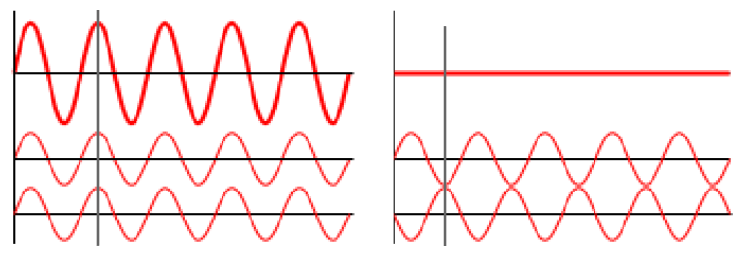
\includegraphics[scale=0.65]{background/interferenceconcept.png}
  \caption[interference]{Interference scenarios$\footnotemark$ when two waves waves meet: On the left hand-side, there is constructive interference and on the right hand-side there is destructive interference illustrated.}
  \label{fig:interferenceconcept}
\end{figure}
\footnotetext{Image source: \texttt{http://en.wikipedia.org/wiki/Interference\textunderscore(wave\textunderscore propagation)} } 

\begin{itemize}
  \item A crest of a wave meets a crest of another wave and similarly a trough meets a trough of another wave. This scenario is denoted as constructive interference and occurs at any location along the medium where the two interfering waves have a displacement in the same direction. This is like saying that the phase difference between the waves is a multiple of $2\pi$. Then the resulting amplitude at that point is being much larger than the amplitude of an individual wave. For two waves with an equal amplitude interfering constructively, the resulting amplitude is twice as large as the amplitude of an individual wave.
  \item A crest of a wave meets a trough of another wave and vice versa. This scenario is denoted as destructive interference and occurs at any location along the medium where the two interfering waves have a displacement in the opposite direction. This is like saying that the phase difference between the waves is an odd multiple of $\pi$. Then the waves completely cancel each other out at any point they superimpose.
  \item If the phase difference between two waves is intermediate between the first two scenarios, then the magnitude of the displacement lies between the minimal and maximal values which we could get from constructive interference.
\end{itemize}

Keep in mind that when two or more waves interfere which each other, the resulting wave may have a different frequency. This means that interfering waves, comming from two light sources with a certain color, may produce a light of another color than they have.

\subsection{Wave Coherence}
\label{sec:wavecoherence}
When considering waves which are traveling on a shared medium along the same direction, we could examine how their phase difference is changing over time. Formulating the change in their relative phase as a function of time will provide us a quantitative measure of the synchronization between those two waves, the so called wave coherence. In order to better understand this concept, let us consider a perfectly mathematical sine wave and a second wave which is a phase-shifted replica of the first one. A property of these mathematical waves is that they keep their shape over an infinity amount of time (i.e. propagated wavelengths). In our scenario, both waves are traveling along the same direction on the same medium, as illustrated in figure $\ref{fig:coherencesinsignal}$.
\begin{figure}[H]
  \centering
  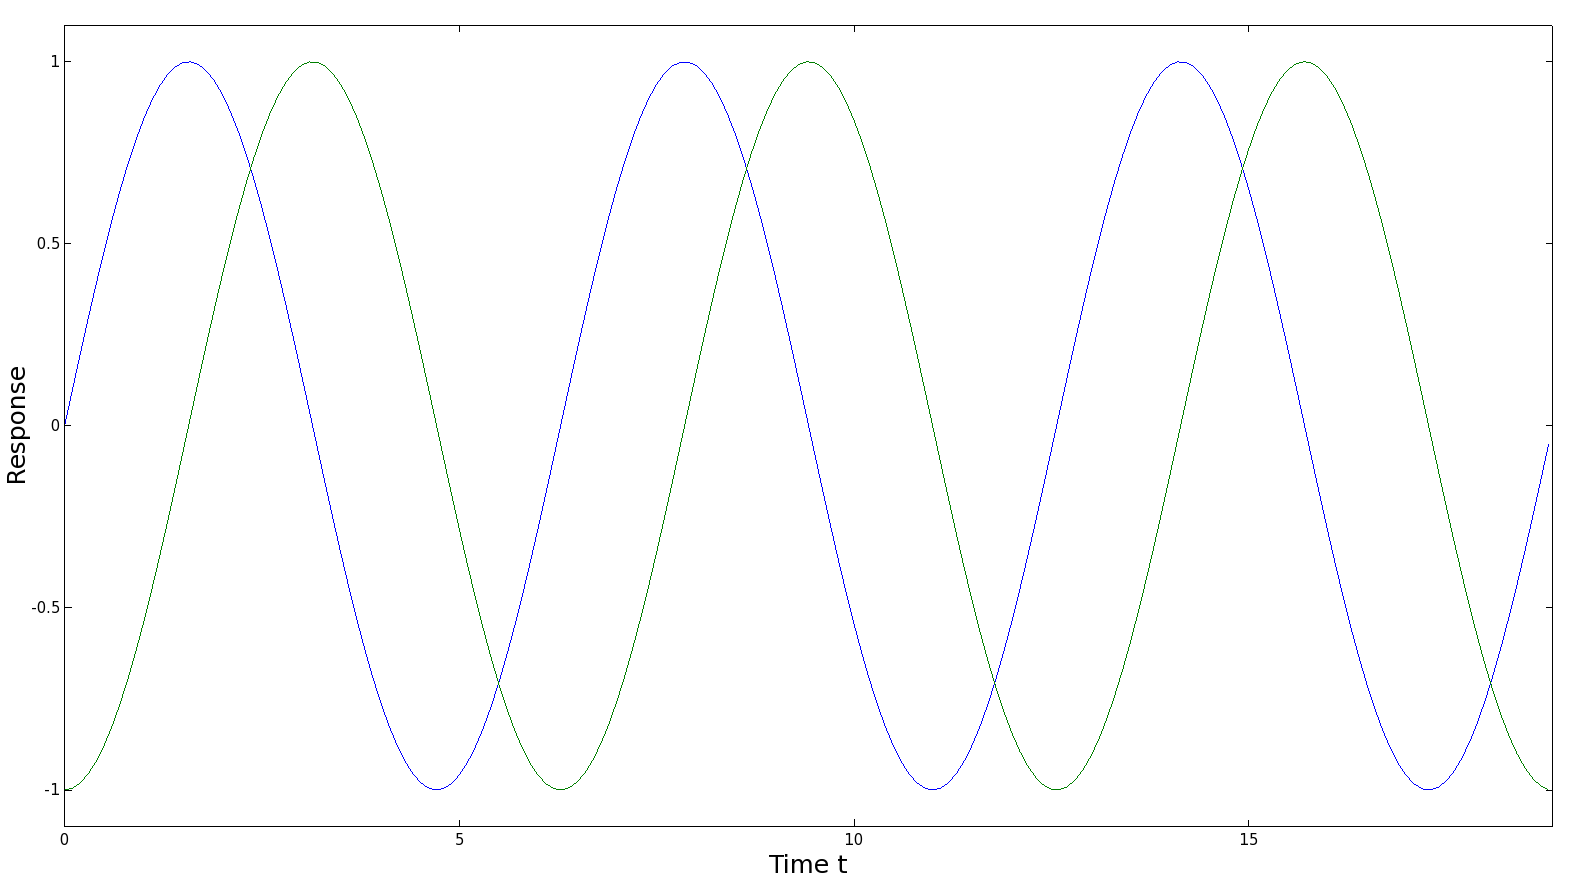
\includegraphics[scale=0.3]{background/coherencesinsignal.png}
  \caption[Wave Coherence]{Two mathematical sine waves which are perfectly coherent which means that their phase difference is constant for every point in time.}
  \label{fig:coherencesinsignal}
\end{figure}
\noindent
Taking the difference between these two sine waves always yields a constant number. Therefore, those two waves are said to be coherent and hence perfectly synchronous over time. Notice that this scenario is completely artificial since in nature there are no mathematical sine waves. Rather, the phase difference is then a function of time $p(t)$. The more coherent two waves are, the slower this function will change over time. 
In fact, two waves are said to be coherent if they are of the same frequency, are temporally in phase or have the same amplitude at every point in time. Thus two waves are coherent if they are generated at the same time, having the same frequency, amplitude, and phase. Conversely, waves are considered incoherent or also asynchronous if they have no stable phase difference. This means $p(t)$ is heavily varying over time. Coherence describes the effect of whether waves will tend to interfere with each other constructively or destructively at a certain point in time and space. Thus this is a property of waves that enables stationary interference. The more correlated two waves are, the higher their degree of coherence is. In physics coherence between waves is quantified by the cross-correlation function, which basically predicts the value of a second wave using the value of the first one. There are two basic coherence classifications:

\begin{itemize}
  \item Spatial coherence is dealing with the question of what is the range of distance between two points in space in the span of a wave for which there is occurring a significant effect of stationary interference when averaged over time. This is formally answered by considering the correlation between waves at different point in space. The range of distance with significant coherence is also denoted as the coherence area.
  \item Temporal coherence examines how well two waves which are observed at two different moments in time correlate with each other. Thus it may be used for predicting how well a wave interferes temporally with itself. Mathematically, this kind of coherence is computed by measuring the correlation between the value of the wave and the delayed version of itself. The coherence time denotes the maximum time delay for which the waves are coherent. The distance a wave has traveled during the coherence time is denoted as their temporal coherence length.
\end{itemize}

\subsection{Huygen's Principle}
\label{sec:huygensprincipledef}
Besides the phases and the amplitudes of waves, their propagation directly affects the interaction between different waves and how they could interfere with each other. This is why it makes sense to formulate a model which allows us to predict the position of a moving wavefront and how it moves in space. This is where $\emph{Huygen's Principle}$ comes into play. It states that any point of a wavefront may be regarded as a point source that emits spherical wavelets in every direction. Within the same propagation medium, these wavelets travel at the same speed as their source wavefront. The position of the new wavefront results by superimposing all of these emitted wavelets. Geometrically, the surface that is tangential to the secondary waves can be used in order to determine the future position of the wavefront. Therefore, the new wavefront encloses all emitted wavelets. Figure $\ref{fig:huygensprinciple}$ visualizes Huygen's principle for a wavefront reflected off from a plane surface.

\begin{figure}[H]
  \centering
  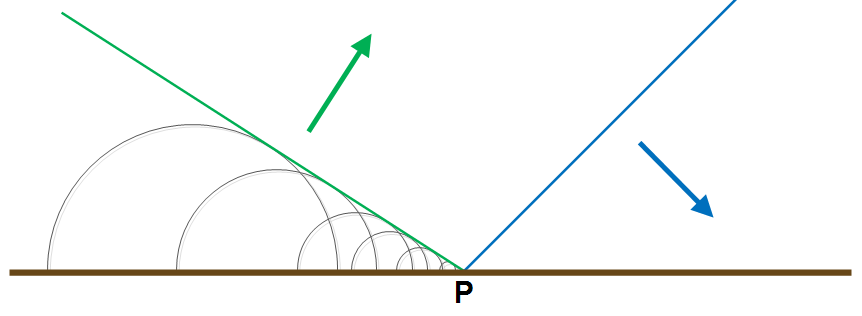
\includegraphics[scale=0.6]{background/huygensprinciple.png}
  \caption[Huygen's Principle]{A moving wavefront (blue) encounters an obstacle (a surface shown in brown colors) and produces a new wavefront (green) as a result of superposition of all secondary wavelets.}
  \label{fig:huygensprinciple}
\end{figure}

\subsection{Waves Diffraction}
Revisting Hugen's Principle we know that each point on a wavefront can be considered as a source of a spherical wavelet which propagates in every direction. But what exactly happens when a wave's propagation direction is only partially occluded by an object? What will be the outcome on applying Huygen's Principle to this case? An example scenario for this case is shown in figure $\ref{fig:wavediffraction}$. 

\begin{figure}[H]
  \centering
  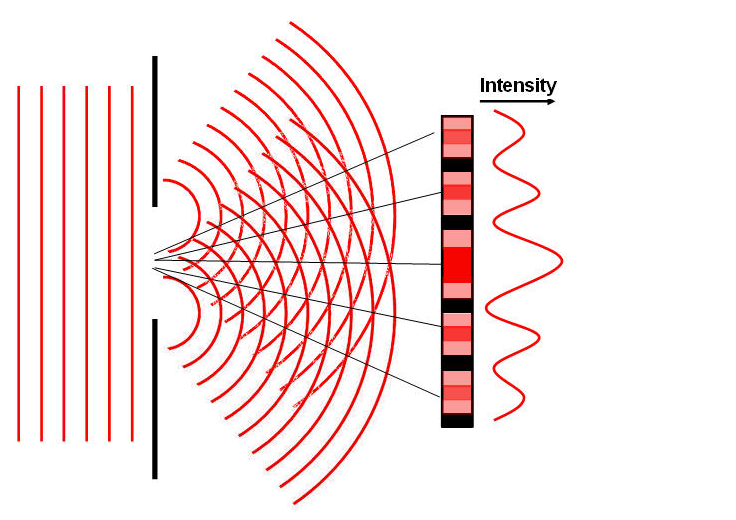
\includegraphics[scale=0.65]{background/diffractiontransmissive.png}
  \caption[Diffracted Wave]{Illustration$\footnotemark$ of a diffraction scenario in which a plane wavefront passes through a surface with a certain width and how the wave will be bent, also showing the intensity of the resulting wave along a straight line in its path.}
  \label{fig:wavediffraction}
\end{figure}
\footnotetext{Image source:\texttt{http://cronodon.com/images/Single\textunderscore slit\textunderscore diffraction\textunderscore 2b.jpg} } 

Whenever a propagating wavefront is partially occluded by an obstacle, the wave is not only moving in the direction along its propagation, but is also bent around the edges of the obstacle. In physics, this phenomenon is called diffraction. Waves are diffracted due to interference which occurs among all wavelets when applying Huygen's Principle for the case when a wavefront hits an obstacle. Generally, the effect of diffraction is most pronounced for the waves whose wavelength is roughly similar in size to the dimension of the occluding object. Conversely, if the wavelength is much smaller in size, then there is almost no wave diffraction perceivable at a far off distance. This relationship between the strength of wave diffraction and the wavelength is conceptually illustrated in figure $\ref{fig:diffractionrelationshipdimension}$ when a wave is transmitted through an opening in a surface. A reflective example for diffraction provided in figure $\ref{fig:huygensprinciple}$.

\begin{figure}[H]
  \centering
  \subfigure[W $\ll$ $\lambda$]{
  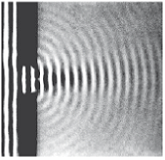
\includegraphics[scale=0.7]{background/Aa2l.png}
    \label{fig:a1}
  }
~
  \subfigure[W $\approx$ $2 \lambda$]{
    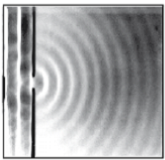
\includegraphics[scale=0.7]{background/Aastl.png}
    \label{fig:a2}
  }
~
  \subfigure[W $\approx$ $6 \lambda$]{
    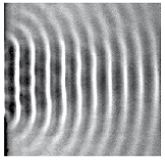
\includegraphics[scale=0.7]{background/Aa6l.png}
    \label{fig:a3}
  }
  \caption[Diffraction for different $\texttt{Wavelength/Slit-Width}$ ratio]{Illustration$\footnotemark$ of how diffraction changes when a wave with wavelength $\lambda$ propagates through a slit of width equal $W$.}
  \label{fig:diffractionrelationshipdimension}
\end{figure}
\footnotetext{Image taken from:\texttt{http://neutrino.ethz.ch/Vorlesung/FS2013/index.php/vorlesungsskript}, chapter 9, figure 9.14 } 

In everyday's life, we can see the direct outcome of the effect of wave diffraction in form of structural colors. There are examples from nature such as the iridescent colors on various snake skins as well as artificial examples such as the colorful patterns notable when having a close look at an illuminated compact disc. All these examples comprise a surface made of highly regular nanostructures which diffract an incident light significantly. Such a nanostructure which exhibits a certain degree of regularity is also denoted as a diffraction grating. Further information about diffraction gratings can be found in section $\ref{sec:diffractiongrating}$.

\section{Stam's BRDF formulation}
\label{sec:sumstam}
The theoretical foundation of this thesis is based on the pioneering work of J.Stam$\cite{diffstam}$ who derived a BRDF formulation to modell the effect of far field diffraction for various analytical anisotropic surfaces, relying on the so called scalar wave theory of diffraction for which a wave is assumed to be a complex valued scalar. It's noteworthy that Stam's BRDF formulation does not take into account the polarization of the incident light. Fortunately, light sources like sunlight and light bulbs are unpolarized. The principal beginhind J. Stam's approach is illustrated in figure $\ref{fig:meaningofstamsapproach}$. 
\begin{figure}[H]
  \centering
  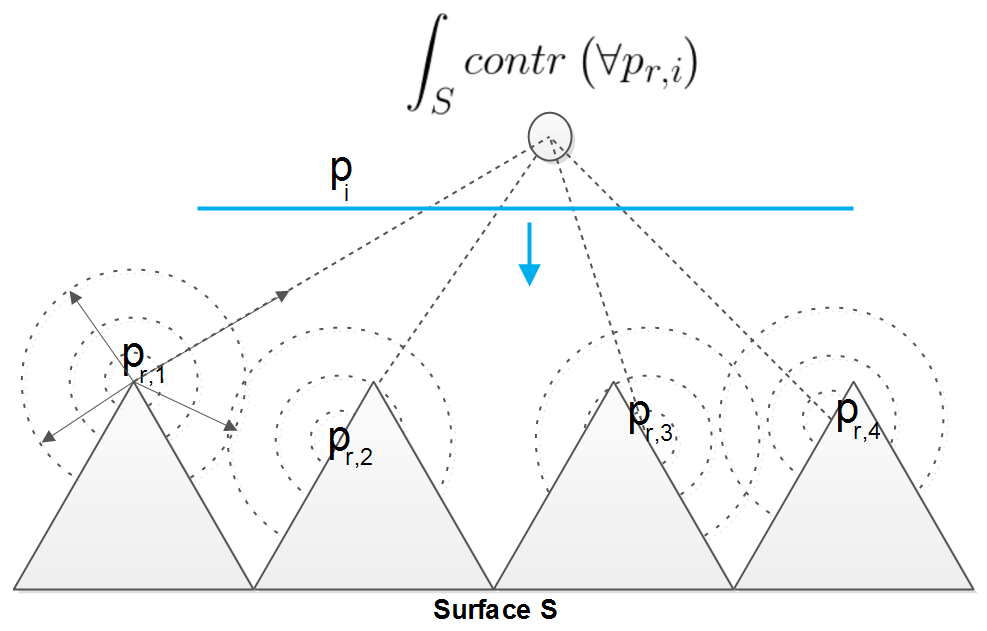
\includegraphics[scale=0.5]{background/stamsapproachsmeaning2.png}
  \caption[Idea behind Stam's approach]{Illustration of secondary wavelets reflected off a surface. An integration over all secondary sources resulting from an incident wave according to Huygen's principle will give us an identity for the total contribution at a certain point in space.}
  \label{fig:meaningofstamsapproach}  
\end{figure}

An incident wave $p_i$ from a a light source encounters a surface representing a diffraction grating. According to Huygen's Principle, at any point $i$ on the grating at which the incident wave meets the grating a secondary, spherical wavelet $p_{r,i}$ will be emitted. A viewer, indicated by a gray circle in the figure, will perceive the superimposed contribution of all wavelets along the surface $S$ (in the figure indicated by a integration symbol), which will directly follow the laws of wave interference. Therefore the resulting color which an observer sees is the final radiance at that point which reflects from stationary interference of all emitted secondary wavelets and per due to Huygen's principle. \\

A further assumption in Stam's Paper is, that the emanated waves from the source are stationary, which implies the wave is a superposition of independent monochromatic waves. This further implies that each wave is associated with a definite wavelength $\lambda$. Directional light sources such as sunlight fulfill this fact and since we are using these kinds of light sources for our simulations, Stam's model can be used for our modelling purposes. \\

% TODO FIX: THIS IS NOT THE MAIN IDEA 
The main model is the formulate a BRDF as the Fourier Transform applied on the given height field, representing a surface like shown in figure $\ref{fig:geometricsetup}$. The classes of surfaces his model is able to support either exhibit a very regular structure or may be considered as a superposition of bumps forming a periodic like structure. Therefore, the surfaces he is dealing with can either be modelled by probabilistic distributions or have a direct analytical representation. Both cases allow him to derive an analytical solution for his BRDF model.

\begin{figure}[H]
  \centering
  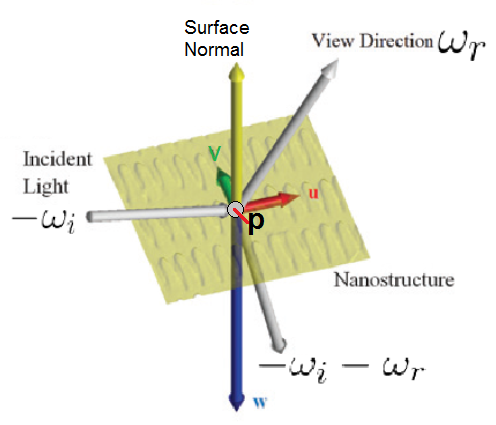
\includegraphics[scale=0.7]{background/stamsinputp.png}
  \caption[Stam's geometrical setup]{Illustration$\footnotemark$ of geometrical setup of Stam's approach where $\omega_i$ is a direction, pointing towards the light source, $\omega_r$ points towards the camera, $n$ is the surface normal, $(u,v,w)$ are the components of the vector $-\omega_i - \omega_r$.}
  \label{fig:geometricsetup}  
\end{figure}
\footnotetext{Modified image which originally has been taken from D.S. Dhillon et. al. poster$\cite{diffourp}$.} 

The direction vector of the secondary wavelet can be computed by taking the difference between the incident and viewing direction like shown in equation $\ref{eq:uvw}$:
\begin{equation}
  (u,v,w) = -\omega_i - \omega_r 
\label{eq:uvw}
\end{equation}
These coordinates will later be used in order to compute the total contribution of all secondary sources used in Stam's BRDF in equation $\ref{eq:mainstam}$. For simplification, let us introduce an auxiliary function $\Phi$ defined in equation $\ref{eq:heightfieldphase}$, which models the phase of a wave from the given height field.

\begin{equation}
  \Phi(x,y) = \frac{2 \pi}{\lambda} w h(x,y) 
\label{eq:heightfieldphase}
\end{equation}

Then, any secondary wavelet $p$ which is emitted off from the given surface is equal:
\begin{equation}
  p(x,y) = e^{i\Phi(x,y)} 
\label{eq:px}
\end{equation}

using the idea presented for figure $\ref{fig:meaningofstamsapproach}$ and performing all mathematical steps shown in the appendix $\ref{chap:stamsderivations}$, will lead us to the final BRDF representation, modelling the total contribution of all secondary sources reflected off the the provided surface $h$ in the direction $\omega_r$:
\begin{equation} 
  BRDF_{\lambda}(\omega_i, \omega_r) = \frac{k^2 F^2 G}{4\pi^2 A w^2} \langle \left|P(ku, kv)\right|^2\rangle
\label{eq:mainstam}
\end{equation}

where $F$ denotes the Fresnel coefficient and $G$ is the so called geometry term$\footnote{The geometric terms expresses the correction factor to perform an integration over an area instead over a surface. For further information, please have a look at \texttt{http://en.wikipedia.org/wiki/Surface\textunderscore integral}, and read the definition about \emph{surface element}}$ which is equal to: 
\begin{equation}
  G =\frac{(1 + \omega_i \cdot \omega_r)^2}{cos(\theta_i)cos(\theta_r)}
\label{eq:geometricterm}
\end{equation}

\label{sec:electricalengeneeringftconvention}
One last word about the Fourier transform terms that Stam uses in his derivation: Conventionally, following the definitions of the Fourier Transformation, we are dealing with the inverse Fourier Transformation. However, especially in electrical engineering, it is quite common to define this inverse Fourier transformation by the Fourier Transformation. The reason behind this lies in the fact that we simply could substitute the minus sign as in the following equation $\ref{eq:signchangementconvention}$:

\begin{align}
\mathcal{F}_{FT}\{f\}(w) 
& = \int_{\mathds{R}^n} f(x)e^{-iwt} dt \nonumber\\
& = \int_{\mathds{R}^n} f(x)e^{i\hat{w}t} dt \nonumber\\
& = \mathcal{F}^{-1}_{FT}\{f\}(\hat{w})
\label{eq:signchangementconvention}
\end{align} 
where $\hat{w}$ is equal $-w$. \\

The height fields we are dealing with in this work are, however, natural gratings containing a complex shaped nano-structure and hence far from being very regularly aligned. The reason why Stam's approach in its current form is not suitable for our purpose is twofold: First his approach does not capture the complexity of natural gratings accurately well enough when relying on his statistical approaches and secondly it is way too slow in order to be usable for interactive rendering since his BRDF needs an evaluation of a Fourier Transform for every directional changing. \\